\subsubsection{Exercise}

The previous controller did not offer good control performance.
Indeed, a loop gain of slope $-1$ at all frequencies gives poor disturbance attenuation. 
It is needed to design a better controller.

\paragraph{Unproper feedback}

As a starting point, we can choose:

$$ F_{y,unproper} = \frac{s + \omega_I}{s} G^{-1} G_d $$

Even if this controller is not proper, we can design $\omega_I$ -- using \texttt{Matlab}. 

Tuning this parameter leads to the following result:
The bigger $\omega_I$ is, the fastest perturbation $d$ is attenuates. 
However, the bigger $\omega_I$ is, the bigger the disturbance becomes.
Therefore we need to find a value which balance this two behaviors.

$\omega_I = 5$ rad/s was the value that gives us the best results: 
        $$|y(t)| \leq 1, \forall t \text{ and } |y(t)| \leq 0.1, \forall t \geq 0.5\text{ s}$$ 

\paragraph{Proper feedback}

As in Exercise \ref{exo421}, the previous controller is not proper.
In order to make it proper, we need to add to poles in $\omega_0$ and $\omega_1$.

Let:

$$ F_{y,proper} = \frac{s + \omega_I}{s} \frac{\omega_0 \omega_1}{(s+ \omega_0)(s + \omega_1)} G^{-1} G_d$$ 

This controller is indeed proper.
As mentioned in the subject, if $G_d \approx 1$, the controller should contain the inverse of the system. 
Since for all $\omega$ in $[0,\omega_c]$, $ G_d \approx 1$, the two poles should be placed \emph{after} $\omega_c$.

We pick:

$$\omega_0 = \omega_1 = 10\omega_I$$

This poles guarantee that the disturbance criteria on $|y(t)|$ is still met.

Figure \ref{designProperFy} display the step response of the system and the response to a step in the disturbance.

\begin{figure}[h!t]
    \centering
    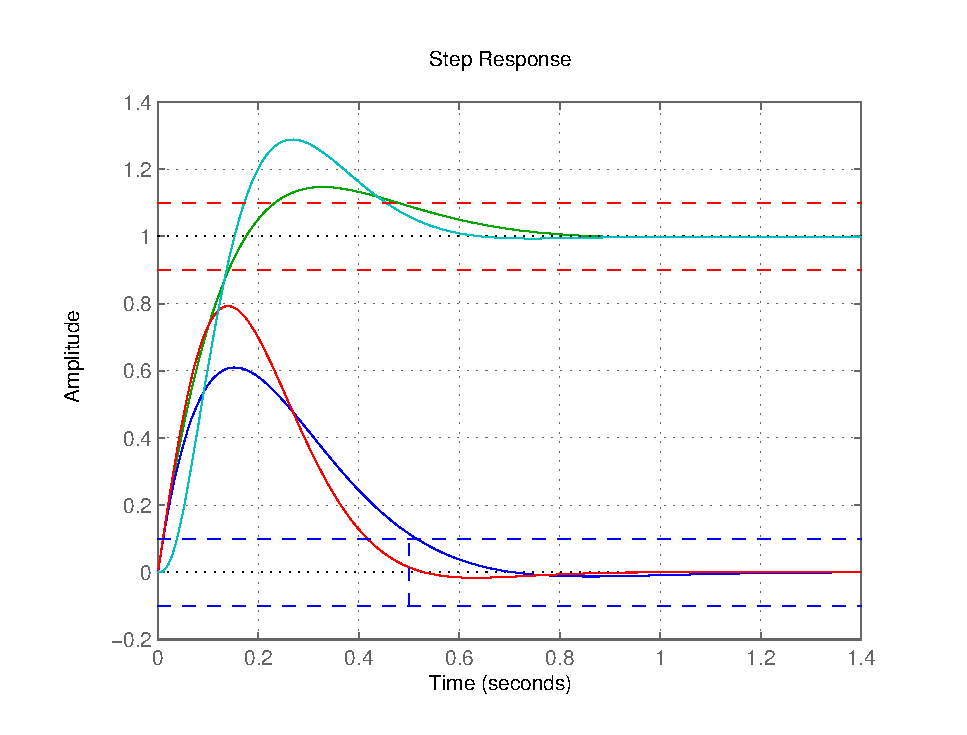
\includegraphics[width=\linewidth]{fig/designProperFy.eps}
    \caption{Step response of the system and response to a step in the disturbance with the proper (red, magenta) and unproper (blue, green) feedback}
    \label{designProperFy}
\end{figure}
